%\subsection{Learning of Weights Given Gates: Refining and Extending Prior Work}\label{sec:analysis}

%In what follows, we first restate the prior result. While \Cref{th:fc} and Theorem 5.1 in \citep{npk} are mathematically identical, \Cref{th:fc} is written in a manner to capture the fact that the NPK is invariant to permutation of the layers. \Cref{th:conv,th:res} are entirely new and are extensions of the dual view for convolutions with global pooling and skip connections. 

\subsection{Theorem Statements}
%\subsection{NPK of FC-DNN: Product Kernel }
%\input{cnpkexample}
%\subsection{Neural Path Kernel : Similarity based on active sub-networks}
%\textbf{Remark.} In the case of fully connected networks, $\textbf{overlap}_{\Theta}(i,x,x')$ is equal for all $i\in[\din]$, and hence $\text{NPK}_{\Theta}(x,x')=\ip{x,x'}\cdot\textbf{overlap}_{\Theta}(x,x')$.
%We point out that this statistical decoupling of weights and gates in \Cref{assmp:main} is unrealisable in a DNN with ReLU, however, this assumption can be trivially realised in a DGN. %Further, we are interested only in the `what?' ( and not `how?') question related to the gates in which case this assumptions is not a restriction.

\begin{theorem}[Product of Kernels Theorem]
\label{th:fc} Under \Cref{assmp:main}  ($\sigma=\frac{\cscale}{\sqrt{w}}$) for FC-DGN : 
\begin{align*}
\text{NTK}_{\text{DGN}}(x,x') \rightarrow d \cdot \cscale^{2(d-1)} \cdot \left(\ip{ x,x'} \cdot \Pi_{l=1}^{d-1} \frac{\ip{G_l(x),G_l(x')}}w\right), \quad\text{as}\,\, w\rightarrow \infty 
\end{align*}
\end{theorem} 
%\textbf{Remark.} Here $\frac{\ip{G_l(x),G_l(x')}}w$ are the \emph{base kernels} measuring the \emph{\textbf{correlation of the gates}}. We show experimentally that the correlation of gates is essentially  `what is learnt in a DNN with ReLUs'.
%and $\Pi_{l=1}^{d-1} \frac{\ip{G_l(x),G_l(x')}}w$ is a product of these base kernels and hence the name `Product of Kernels Theorem'.  The base kernels are essentially measuring which we show via  We now list the roles of the two networks, weights, depth and width.

%\textbf{Feature Network.} The role of this network is to process the input layer-by-layer and produce the $w$-dimensional gating features $G_l(\cdot)$. Each layer comprises of `$w$' ReLUs, and a given ReLU (i.e., gate) is `on' if the input to that layer lies on the positive half-space of hyperplane of given by the incoming weights of that ReLU. Thus the gates of a given layer are based on the angle between the input to that layer and the various hyperplanes given by the weights of that layer. Prior experiments in [\citenum{npk}] and the experiments in this paper show that the feature network, i.e., the gates hold most information, which in turn means that weights of the feature network are key.

%\textbf{Value Network}. The value network implements the product of kernels by laying out the gates as masks depth-wise, and connecting them in the structure of a DNN. Note that depth-wise layout plays an important role here: for instance, if we were to concatenate the gating features as $\varphi(x)=(G_l(x),l=1,\ldots,d-1)\in\{0,1\}^{(d-1)w}$, it would have only resulted in the kernel $\ip{\varphi(x),\varphi(x')}=\sum_{l=1}^{d-1}{\ip{G_l(x),G_l(x')}}$, i.e., a \emph{sum  (not product)} of kernels. Prior experiments in [\citenum{npk}] and the experiments in this paper show that the value network can be reset and re-trained without loss of performance, which in turn means that weights of the value network are not that important.

%\textbf{Note.} The above insights from \Cref{th:main} carry over to the case of DNN with ReLUs by thinking that the roles of value and feature network are performed by a single network.

\textbf{Convolutions with pooling.} Let the circular rotation of vector $x\in\R^{\din}$ by `$r$' co-ordinates be defined as $rot(x,r)(i)=x(i+ r)$, if $i+r \leq \din$ and $rot(x,r)(i)=x(i+ r-\din)$ if $i+r > \din$. Using circular convolutions with pooling results in a rotationally invariant kernel \Cref{th:mainconv}. The architecture and the notations for the network with convolutions is presented in the Appendix.
\begin{comment}
 We extend the dual view to neural network with $\dc$ convolutional layers ($l=1,\ldots,\dc$), followed by a \emph{global-average/max-pooling} layer ($l=\dc+1$) and $\dfc$ ($l=\dc+2,\ldots,\dc+\dfc+1$) fully connected  layers (see Appendix for notation). The convolutional window size is $\wconv<\din$, the number of filters per convolutional layer as well as the width of the fully connected layers is $w$. The main steps are (i) treating pooling layers like gates/masks, (ii) bundling together the paths that share the same path value (due to weight sharing in convolutions) and (iii) re-defining the NPF and NPV for these bundles. The important consequence of weight sharing (due to convolutions and pooling) is that the NPK becomes rotationally invariant resulting in \Cref{th:mainconv}.
\end{comment}
\begin{theorem}[Rotationally Invariant Kernel Theorem]\label{th:conv} Under \Cref{assmp:main}, for  a suitable $\bcnn$:
\begin{align*}
&\kv_{\Tdgn_0}&\ra&\quad \frac{\bcnn}{{\din}^2} \cdot \sum_{r=0}^{\din-1} \ip{x,rot(x',r)}_{\Lambda(\cdot, x,rot(x',r))},\,\, \text{as}\,\,  w\ra\infty\,\text{(for global-average-pooling)}, \\
&\kv_{\Tdgn_0}&\ra& \quad{\bcnn} \cdot \sum_{r=0}^{\din-1} \ip{x,rot(x',r)}_{\Lambda(\cdot, x,rot(x',r))},\,\, \text{as}\,\,  w\ra\infty\,\text{(for global-max-pooling)}
\end{align*}
\end{theorem}

\textbf{Residual Networks with Skip connections.} We consider a ResNet with `$(b+2)$' blocks and `$b$' skip connections between the blocks (left of \Cref{fig:resnet}). Each block is a fully connected (FC) DNN of depth `$\dblock$' and width `$w$'. There are combinatorially many sub-FC-DNNs within this ResNet (see \Cref{def:subfcdnn} and right of \Cref{fig:resnet}).
%\FloatBarrier
\begin{figure}[t]
\begin{minipage}{0.5\columnwidth}
\resizebox{\columnwidth}{!}{
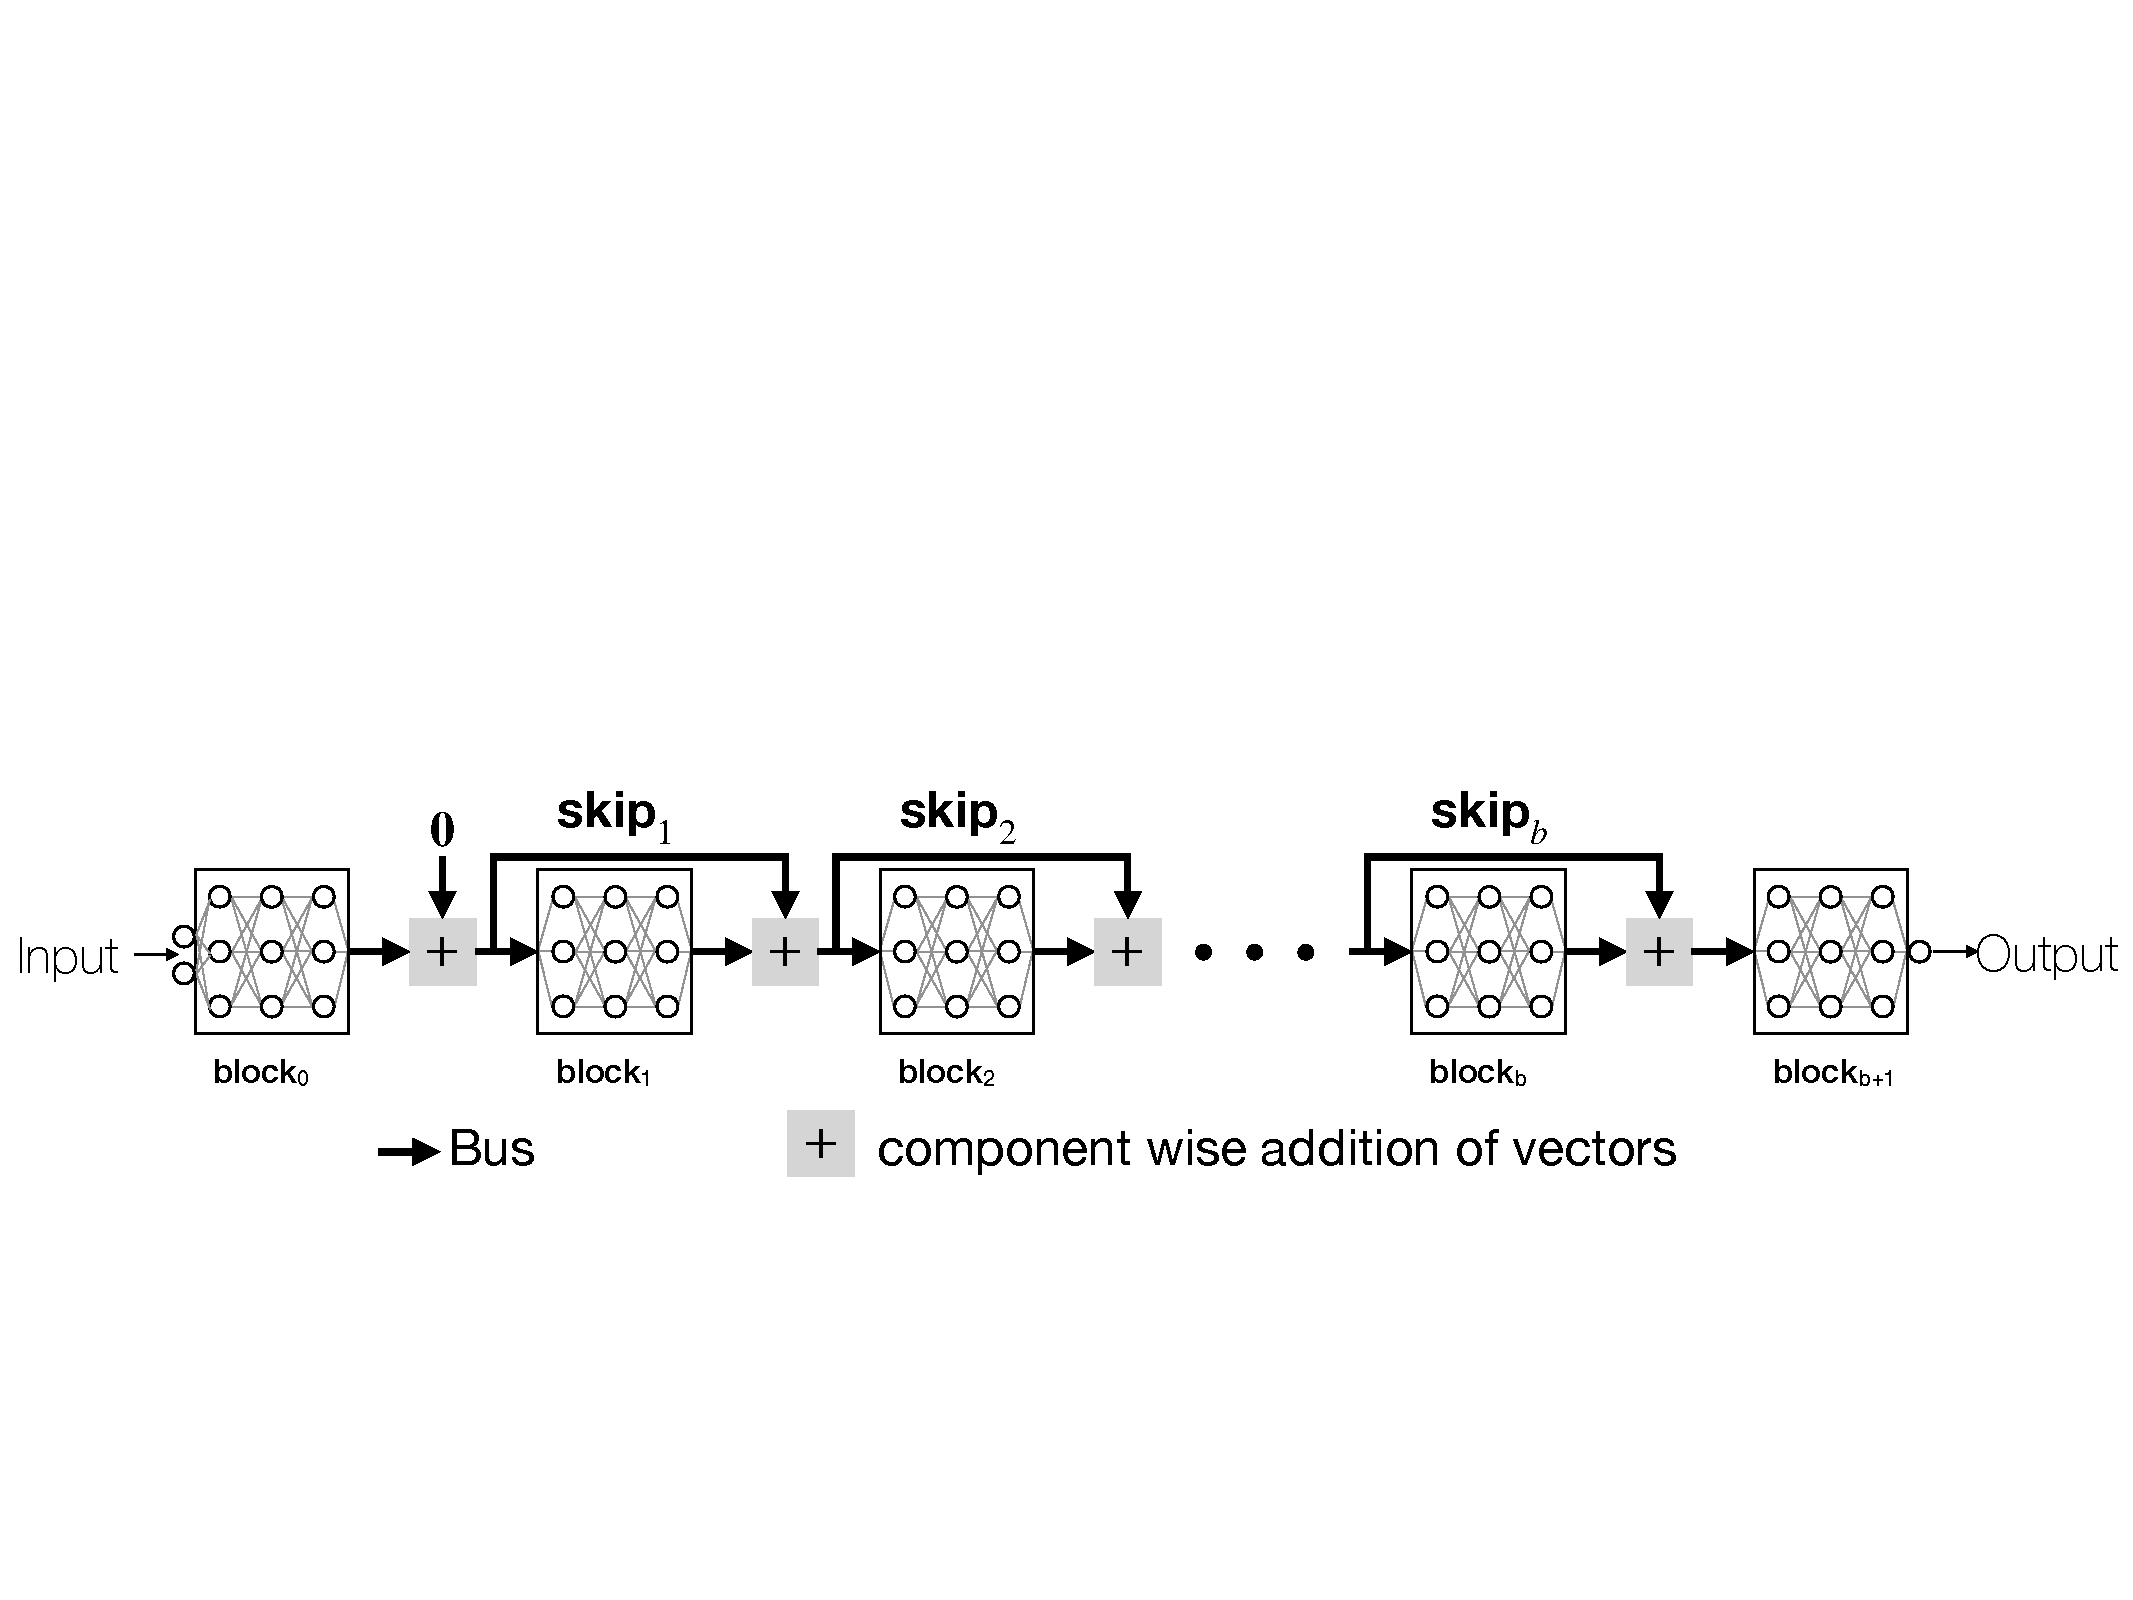
\includegraphics[scale=0.5]{figs/resnet.pdf}
}
\end{minipage}
\begin{minipage}{0.5\columnwidth}
\resizebox{\columnwidth}{!}{
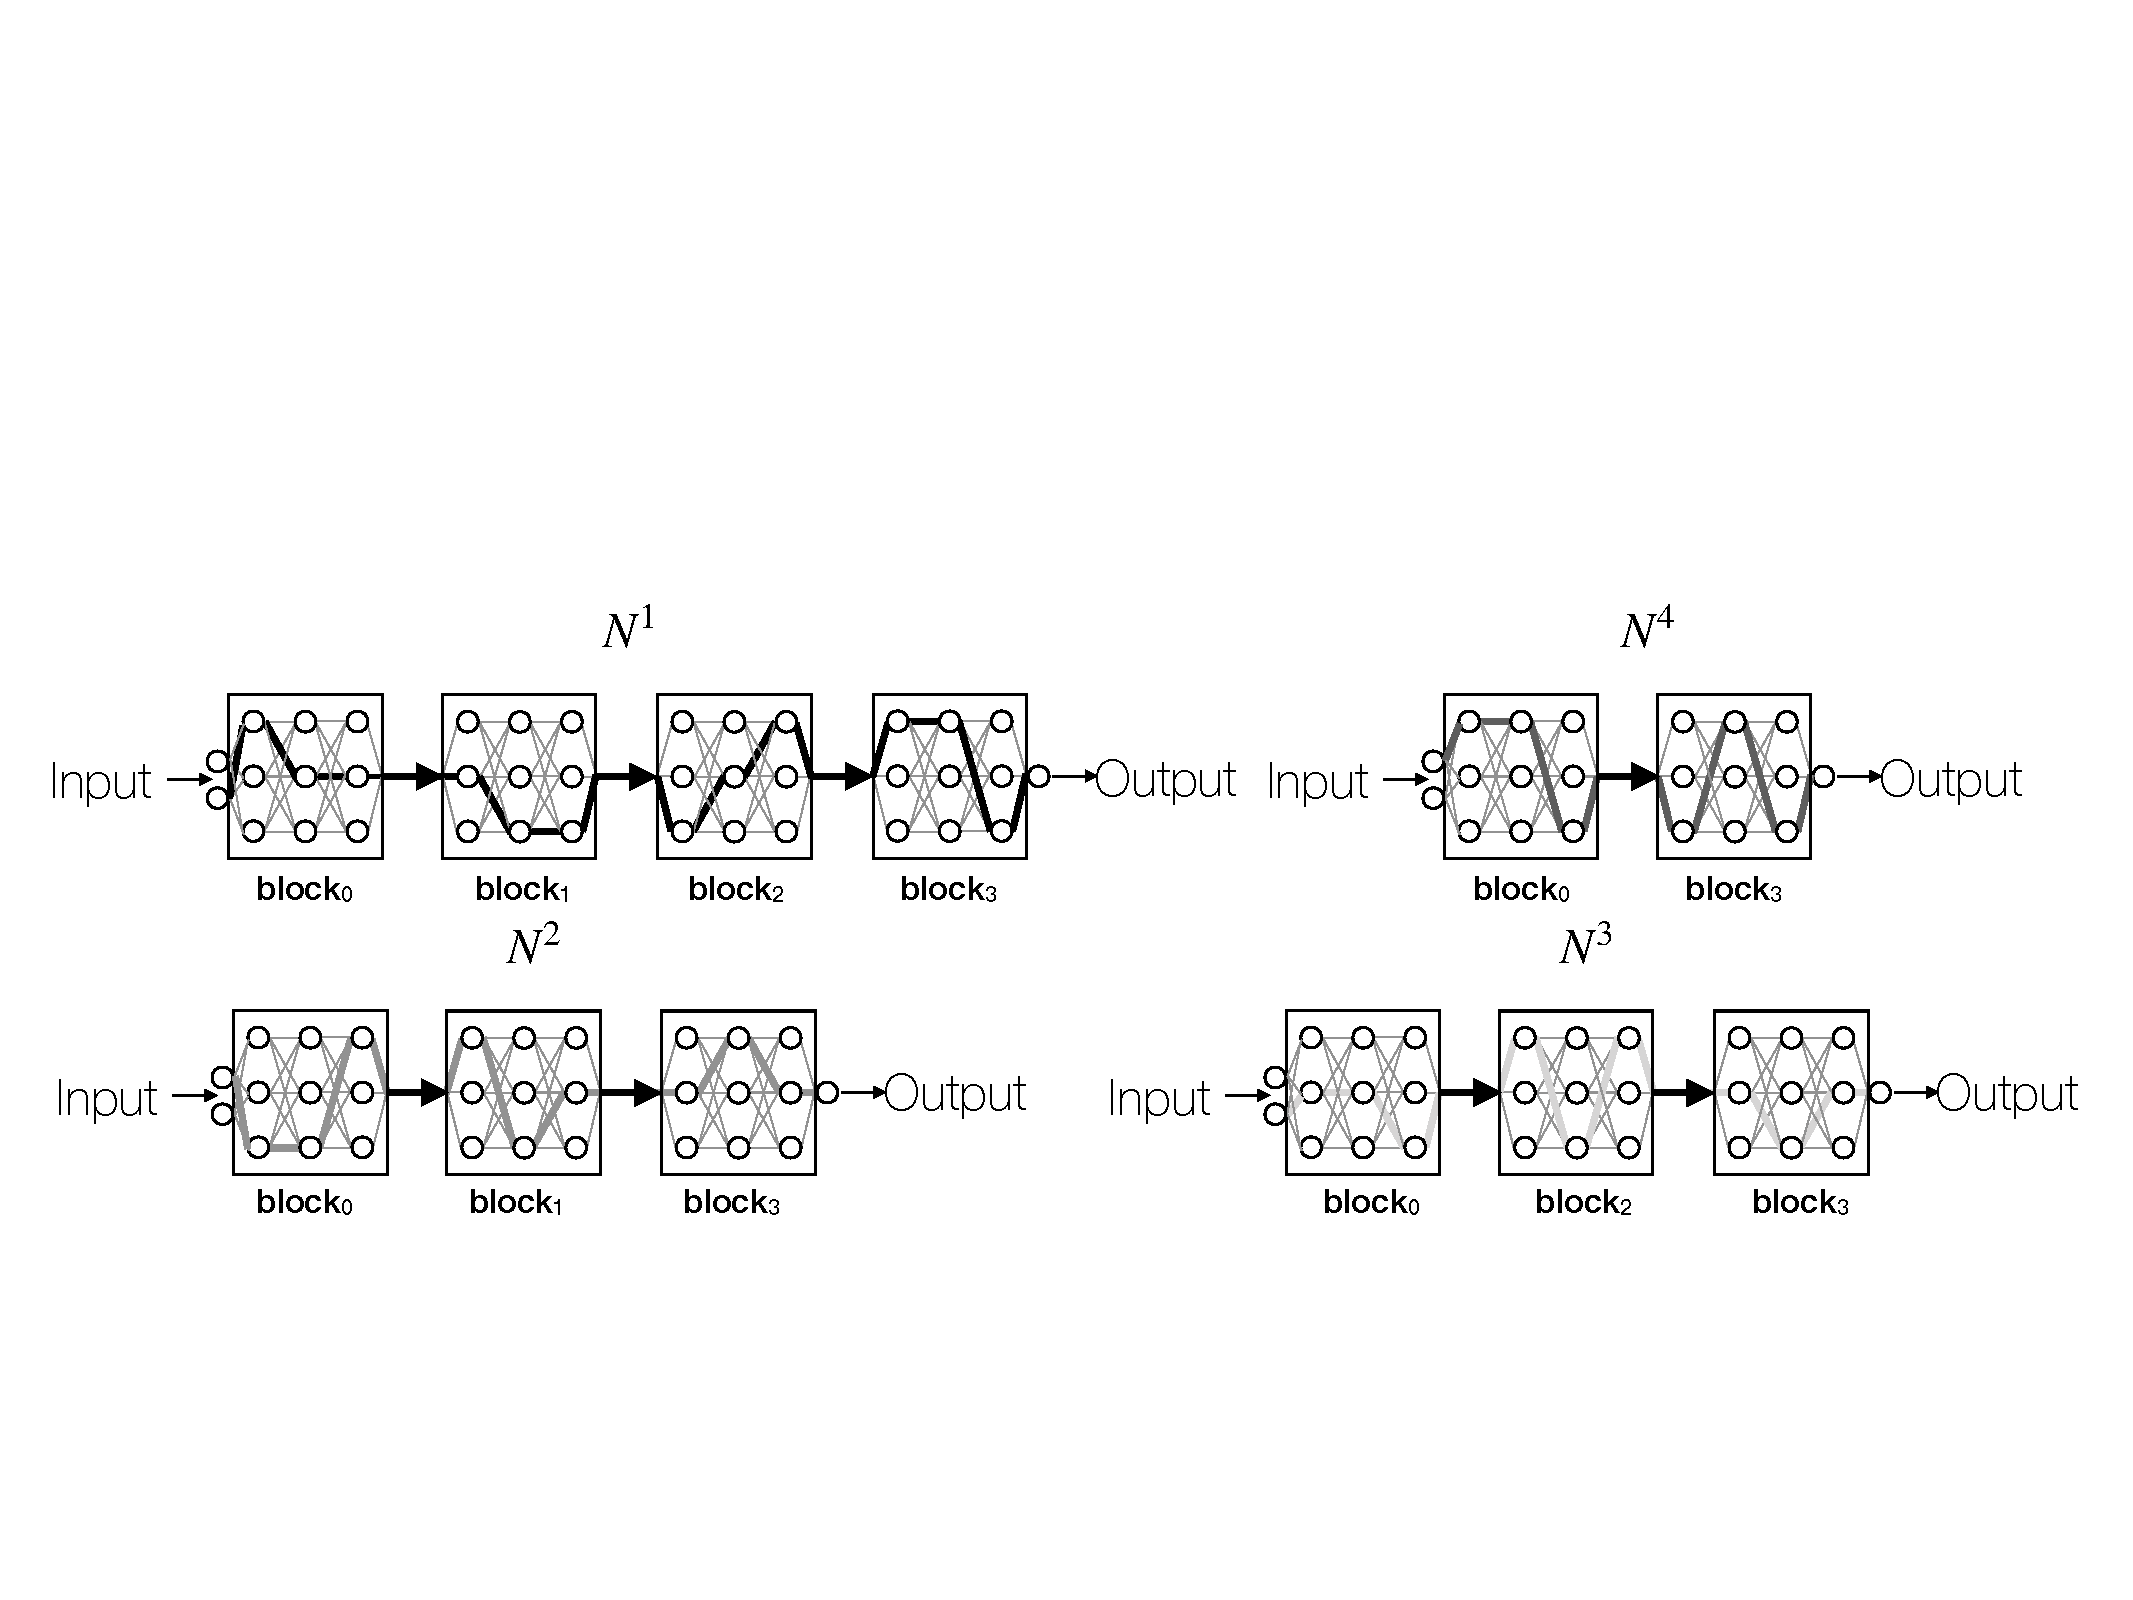
\includegraphics[scale=0.5]{figs/blocks.pdf}
}
\end{minipage}
\caption{\small{On the left is the ResNet with $b$ skip connections and $(b+2)$ blocks. On the right are the sub-FC networks $N^1$ obtained by skipping no blocks, $N^2$ and $N^4$ obtained by skipping block $1$ and $2$ respectively, and $N^3$ obtained by skipping both blocks $1$ and $2$.}}
\label{fig:resnet}
\end{figure}

\begin{definition}\label{def:subfcdnn}[Sub FC-DNNs]
Let $2^{[b]}$ denote the power set of $[b]$ and let $\J\in 2^{[b]}$ denote any subset of $[b]$. Define the`$\J^{th}$' sub-FC-DNN of the ResNet to be the fully connected network obtained by (i) including  $\text{block}_{j},\forall j\in \J$  and (ii) ignoring $\text{block}_{j},\forall j\notin \J$ (see \Cref{fig:resnet}).
\end{definition}
\begin{theorem}
[Sum of Product of Kernels Theorem]\label{th:res} Let $H^{\J}_{\Tf_0}$ be the NPK of the $\J^{th}$ sub-FC-DNN, and $\bfc^{\J}$ be the associated constant. Under \Cref{assmp:main}, we have:
\begin{align*}
\kv_{\Tdgn_0}\ra \sum_{\J\in 2^{[b]}}  \bfc^{\J} H^{\J}_{\Tf_0}, \,\, \text{as}\,\,  w\ra\infty
\end{align*}
\end{theorem}
\textbf{Note.} The sub-FC-DNNs we refer to in \Cref{th:mainres} belong to (or are parts of) the feature network from which the gates are obtained. 

$\bullet$ In \Cref{th:conv} $\sum_{r=0}^{\din-1} \ip{x,rot(x',r)}_{\Lambda(\cdot, x,rot(x',r))}=\sum_{r=0}^{\din-1} \left(\sum_{i=1}^{\din} x(i) rot(x',r)(i)\Lambda(i,x,x')\right)$, where the inner `$\Sigma$' is the inner product between $x$ and $rot(x',r)$ weighted by $\Lambda$ and the outer `$\Sigma$' covers all possible rotations, which results in the rotational invariance property. The rotational invariance property holds for architectures using convolutional layer only in the presence of global-pooling. It was observed in the experiments of \cite{arora2019exact} that networks with global-average-pooling are better than vanilla convolutional networks. That said, the rotational invariance property of the kernel is not a new observation in this paper; It was shown by \cite{li2019enhanced} that  prediction using CNTK-GAP is equivalent to prediction using CNTK without GAP but with full translation data augmentation with wrap-around at the boundary. However, \Cref{th:conv} is a necessary result, in that, it demonstrates that this rotational invariance property is recovered in the dual view as well. We also note here that the rotational invariance property continues to hold even if we provide a constant $\mathbf{1}$ input and also destroy the layer-by-layer structure, which are novel insights that naturally follow from the dual path-by-path formulation.

%In order to completely address the `black box'-ness issue, an ideal goal is to aim for theoretical results (supported by empirical evidence) on finite time learning in finite width \texttt{DGN-NO-ACT}. We find this goal is too hard at this stage and do not pursue the same. The next level is to analyse  the primal linearity and the dual linearity separately. Understanding the primal linearity has two parts to it (i) `what do the learnt pre-activations mean?', and (ii) `how are useful pre-activations learnt?'. The `what' question is \emph{post-hoc}, i.e., we can inspect the learnt pre-activations after training. However, we believe that in order to obtain domain specific insights on what the learnt pre-activations mean, we might require domain specific tools. For instance, in the case of `image classification', the pre-activations are the result of series of convolutions by `filter banks', and in order to do full justice, any visual interpretation should also tally with the results from `filter bank' theory. We defer the `what' question for future work. We also believe new theory is required to answer `how are useful pre-activations learnt?', and defer the same to future work. In this paper,  


%$\bullet$ We empirically show that \texttt{DGN-NO-ACT} performs comparably well on standard datasets. 

%$\bullet$ We restate the prior result for the fully connected case so as to explicitise the role of gates, depth and width. We extend the dual view theory to cover  convolutions with global pooling and skip connections.  We show empirically that the value network learns path-by-path and not layer-by-layer.




%A \texttt{DGN-NO-ACT} learns the relation $\hat{y}(x)=\ip{\phi_\Tf(x),v_{\Tv}}$, by learning simultaneously the feature and value network parameters. The pre-activations generated by the feature network trigger the gates thereby directly dictating the neural path feature $\phi_\Tf(x)$. It was shown that neural path features (i.e., the gates) are learnt during training and such learning improves generalisation \cite{npk}. Thus, while the learning in feature network is key, we reserve its theoretical study for future work. In this section, we will analyse the dual linearity, wherein, the theoretical results are in the \emph{inifinite width regime} which yield us a \emph{kernel} interperation, using which we probe into the properties of finite width networks. In other words, our aim is not to propose pure kernel methods with the kernel derived from an inifnite width DNN. 

%For the purpose of analysing the dual, we first explicitise in \Cref{th:fc} an unnoticed invariance property in the prior result of \cite{npk} for fully connected networks. In \Cref{th:conv,th:res} we also extend the dual formulation to cover the cases of convolutions with global pooling and skip connections. These results justify the constant $\mathbf{1}$ input to the value network of the \texttt{DGN-NO-ACT}. We also experimentally verify the constant $\mathbf{1}$ input as well as destroying the layer-by-layer structure of the gates does not degrade the performance. While these results are surprising and counter intuitive with respect to the primal view, they are follow in a straightforward manner from the results in the dual view, thereby underscoring the fact the value network indeeed computes path-by-path, and eliminating the `mystery' as to whether sophisticated structures are learnt layer-by-layer.

\section{Numerical Experiments}\label{sec:exp} 
In what follows, \Cref{sec:exp1} is themed around the key insight obtained from \Cref{th:main}, i.e., the correlation of the gates lies at the heart of `what is learnt in a DNN with ReLUs'. In particular, we show that operations (such as permuting the layers, tiling cum rotation of the gates, and giving a constant `all-ones' input to the value network) that destroy the layer by layer computational structure do not degrade test performance. These operations lead to combinatorially many models and in all of them the test performance remains the same. In \Cref{sec:exp2} we throw light on the open question in [\citenum{randlabel}] on why test performance degrades due to upstream training with random labels. 
\subsection{Robustness of Gates: Destroying layer-by-layer structure does not affect performance}\label{sec:exp1}
In this experiment we show that information in the gates is invariant even if we destroy the layer-by-layer structure. We consider the three kinds of gates (or gating regimes) described below.\\
%\indent \quad$1.$ \textbf{Fixed Learnt:} We \emph{pre-train} the feature network (which is a DNN with ReLUs), then \emph{freeze} the weights of the feature network, and then train the value network. This way we can measure information in the gates of a trained DNN.\\
%\indent \quad$2.$ \textbf{Fixed Random:} We initialise the feature network at random, and then \emph{freeze} its weights and then train the value network. This way we can measure information in the gates of a DNN at initialisation. Here, the feature and value network can be either initialised with the same weights i.e., dependent initialisation (DI) or statistically independent weights  i.e., independent initialisation (II).\\
%\indent \quad$3.$ \textbf{Decoupled Learning:} We initialise the weights of the value and feature network statistically independent and then train both of them. For the gradient to flow through the feature network we use \emph{soft-gating}, i.e., $G(q)=\frac{1}{1+\exp({-\beta\cdot q})}$, with $\beta=10$. 

We make use of the deep gated network (DGN) setup shown in \Cref{fig:dgn-prior-new} (right) which is an improvisation of the DGN in prior work [\citenum{npk}] shown in \Cref{fig:dgn-prior-new} (left). In the current setup, {\bf{$G_{i_1},\ldots,G_{i_4}$ is a permutation of the $G_1,\ldots,G_4$}}, which gives $24$ models. Note that these \textbf{permutations destroy the layer by layer structure}. In the prior setup both value and feature networks have the same input $x\in\R^{\din}$. In the current setup, we have two separate inputs, $x^{\text{f}}\in\R^{\din}$ for the feature network and $x^{\text{v}}\in\R^{\din}$ for the value network. We set $x^{\text{f}}=x$ always, however, for $x^{\text{v}}$ there are \textbf{two modes} namely (i) \textbf{standard}: we set $x^{\text{v}}=x$ ,(ii) \textbf{`all-ones'}: we set $x^{\text{v}}=\mathbf{1}\in\R^{\din}$ (a tensor of all $1$'s). While the setup on the left is only one model, the setup on the right has $\mathbf{48=24\times 2}$ \textbf{different models}, where $24=\texttt{factorial}(4)$ is due to the gate permutations and $2$ is due the settings of $x^{\text{v}}$.
\begin{figure}[t]
\centering
\begin{minipage}{0.4\columnwidth}
\centering
\resizebox{\columnwidth}{!}{
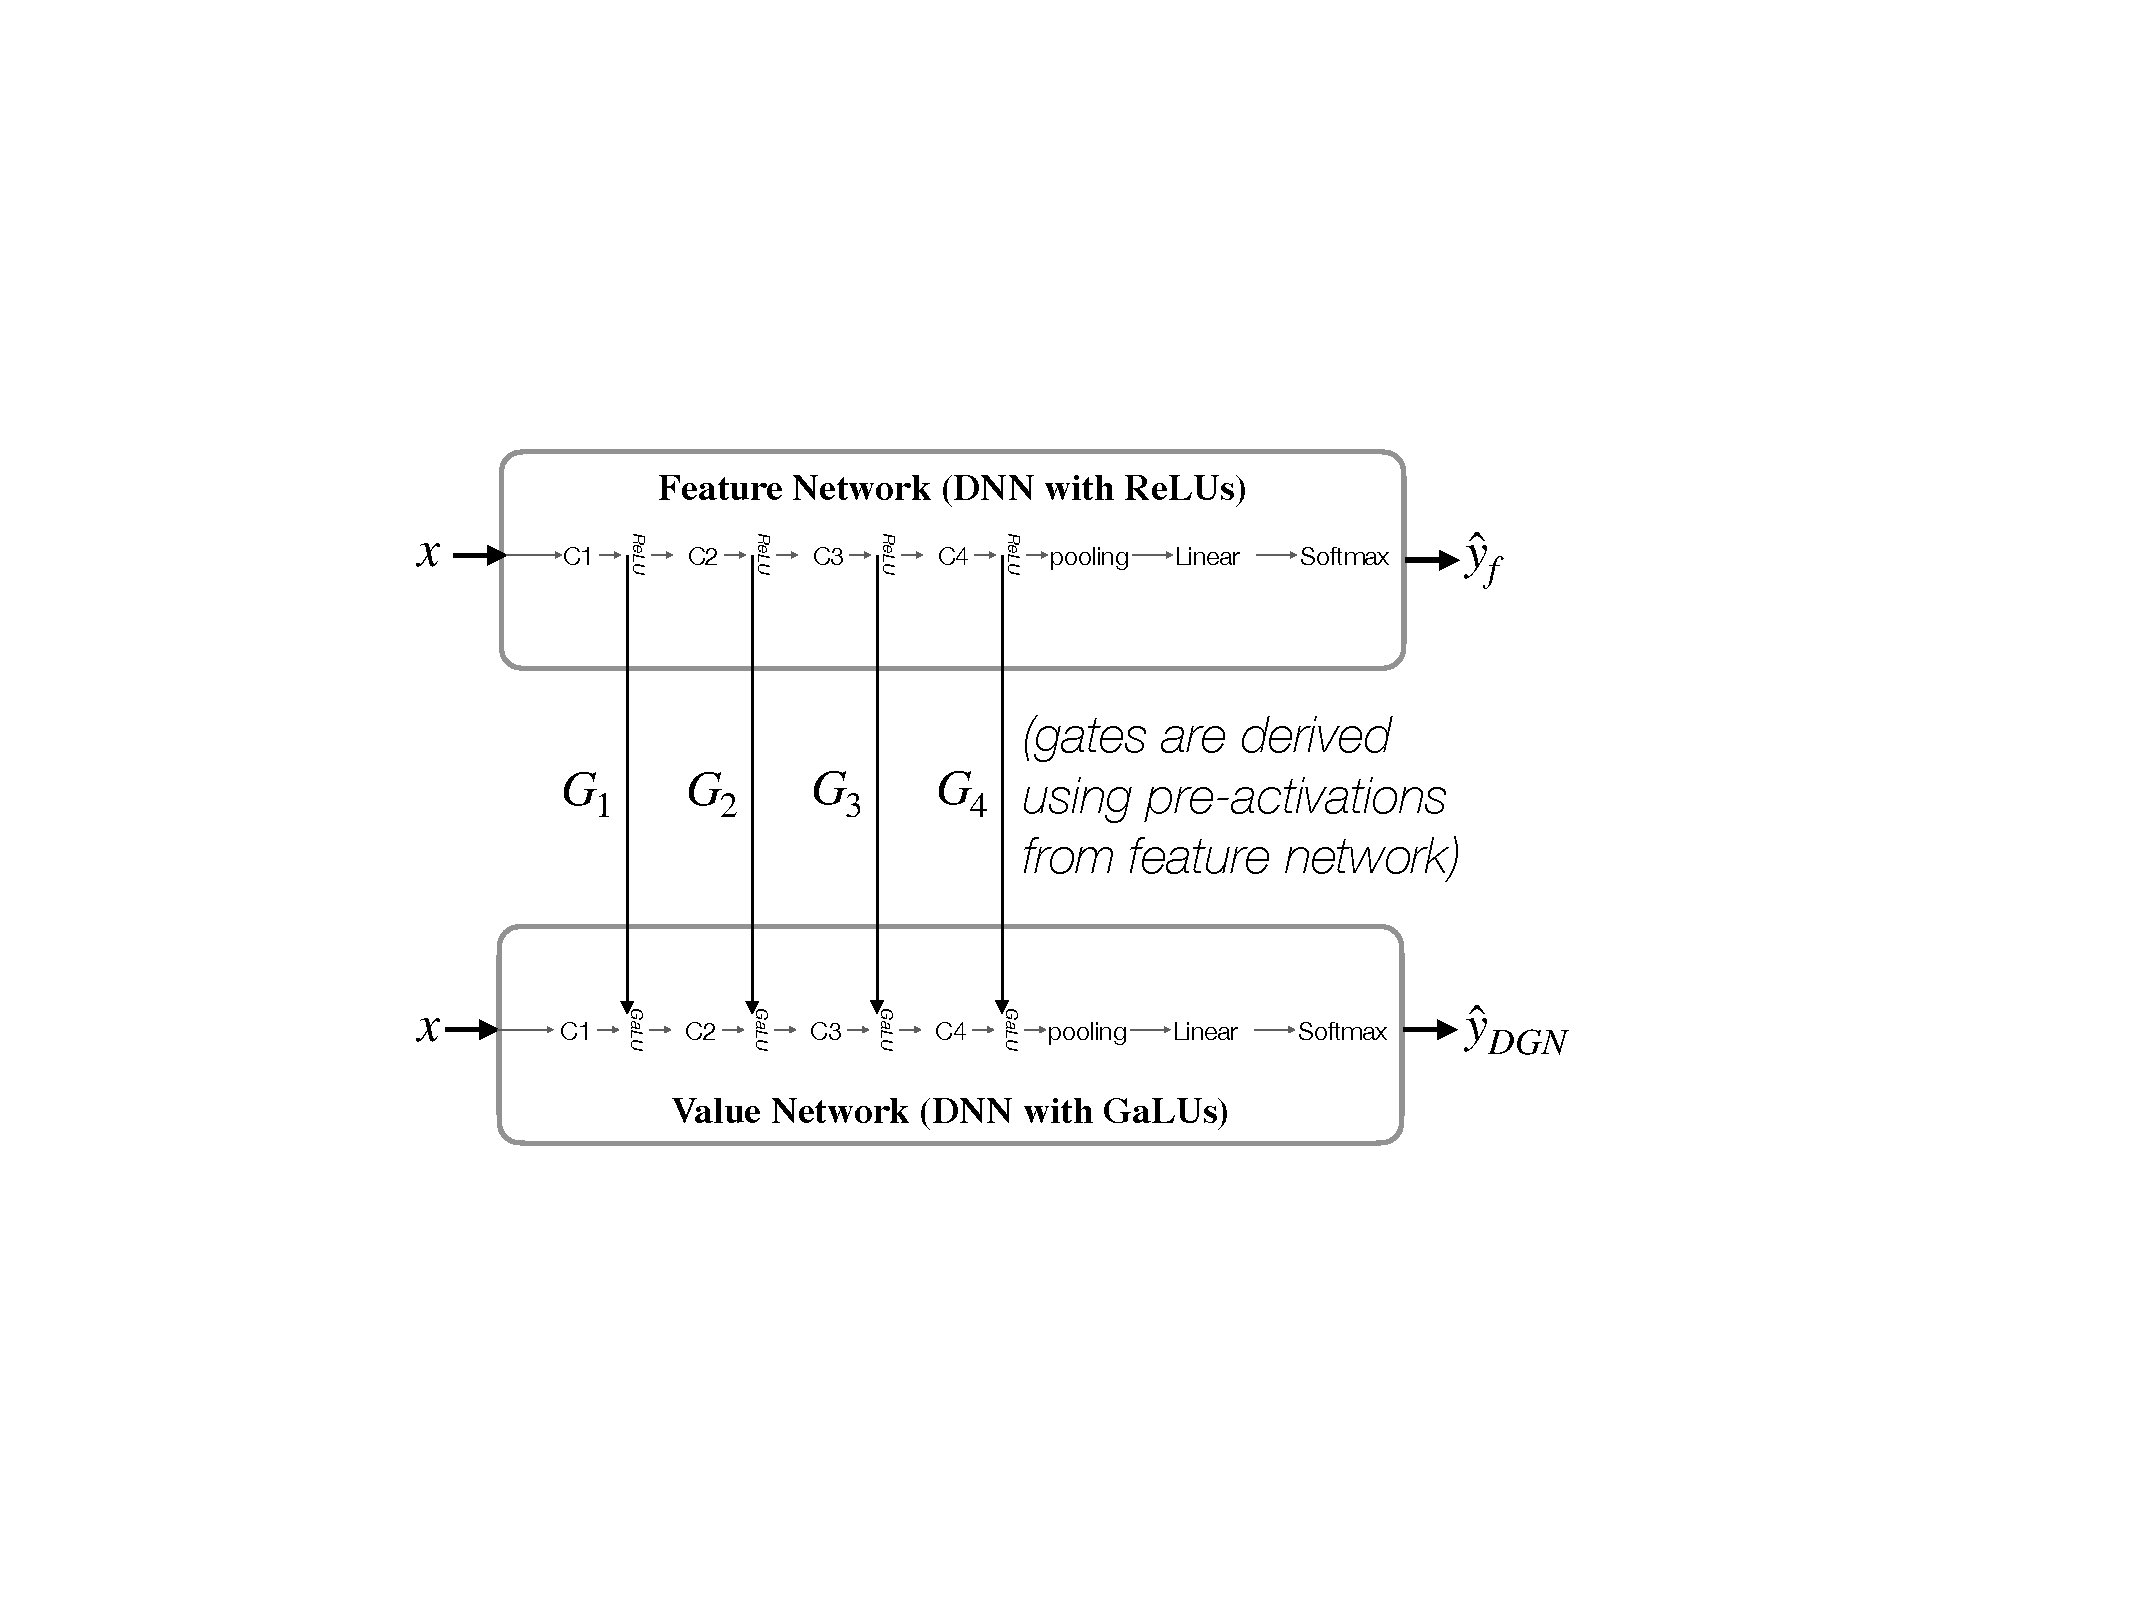
\includegraphics[scale=0.3]{figs/exp-prior.pdf}
}
\end{minipage}
\begin{minipage}{0.4\columnwidth}
\centering
\resizebox{\columnwidth}{!}{
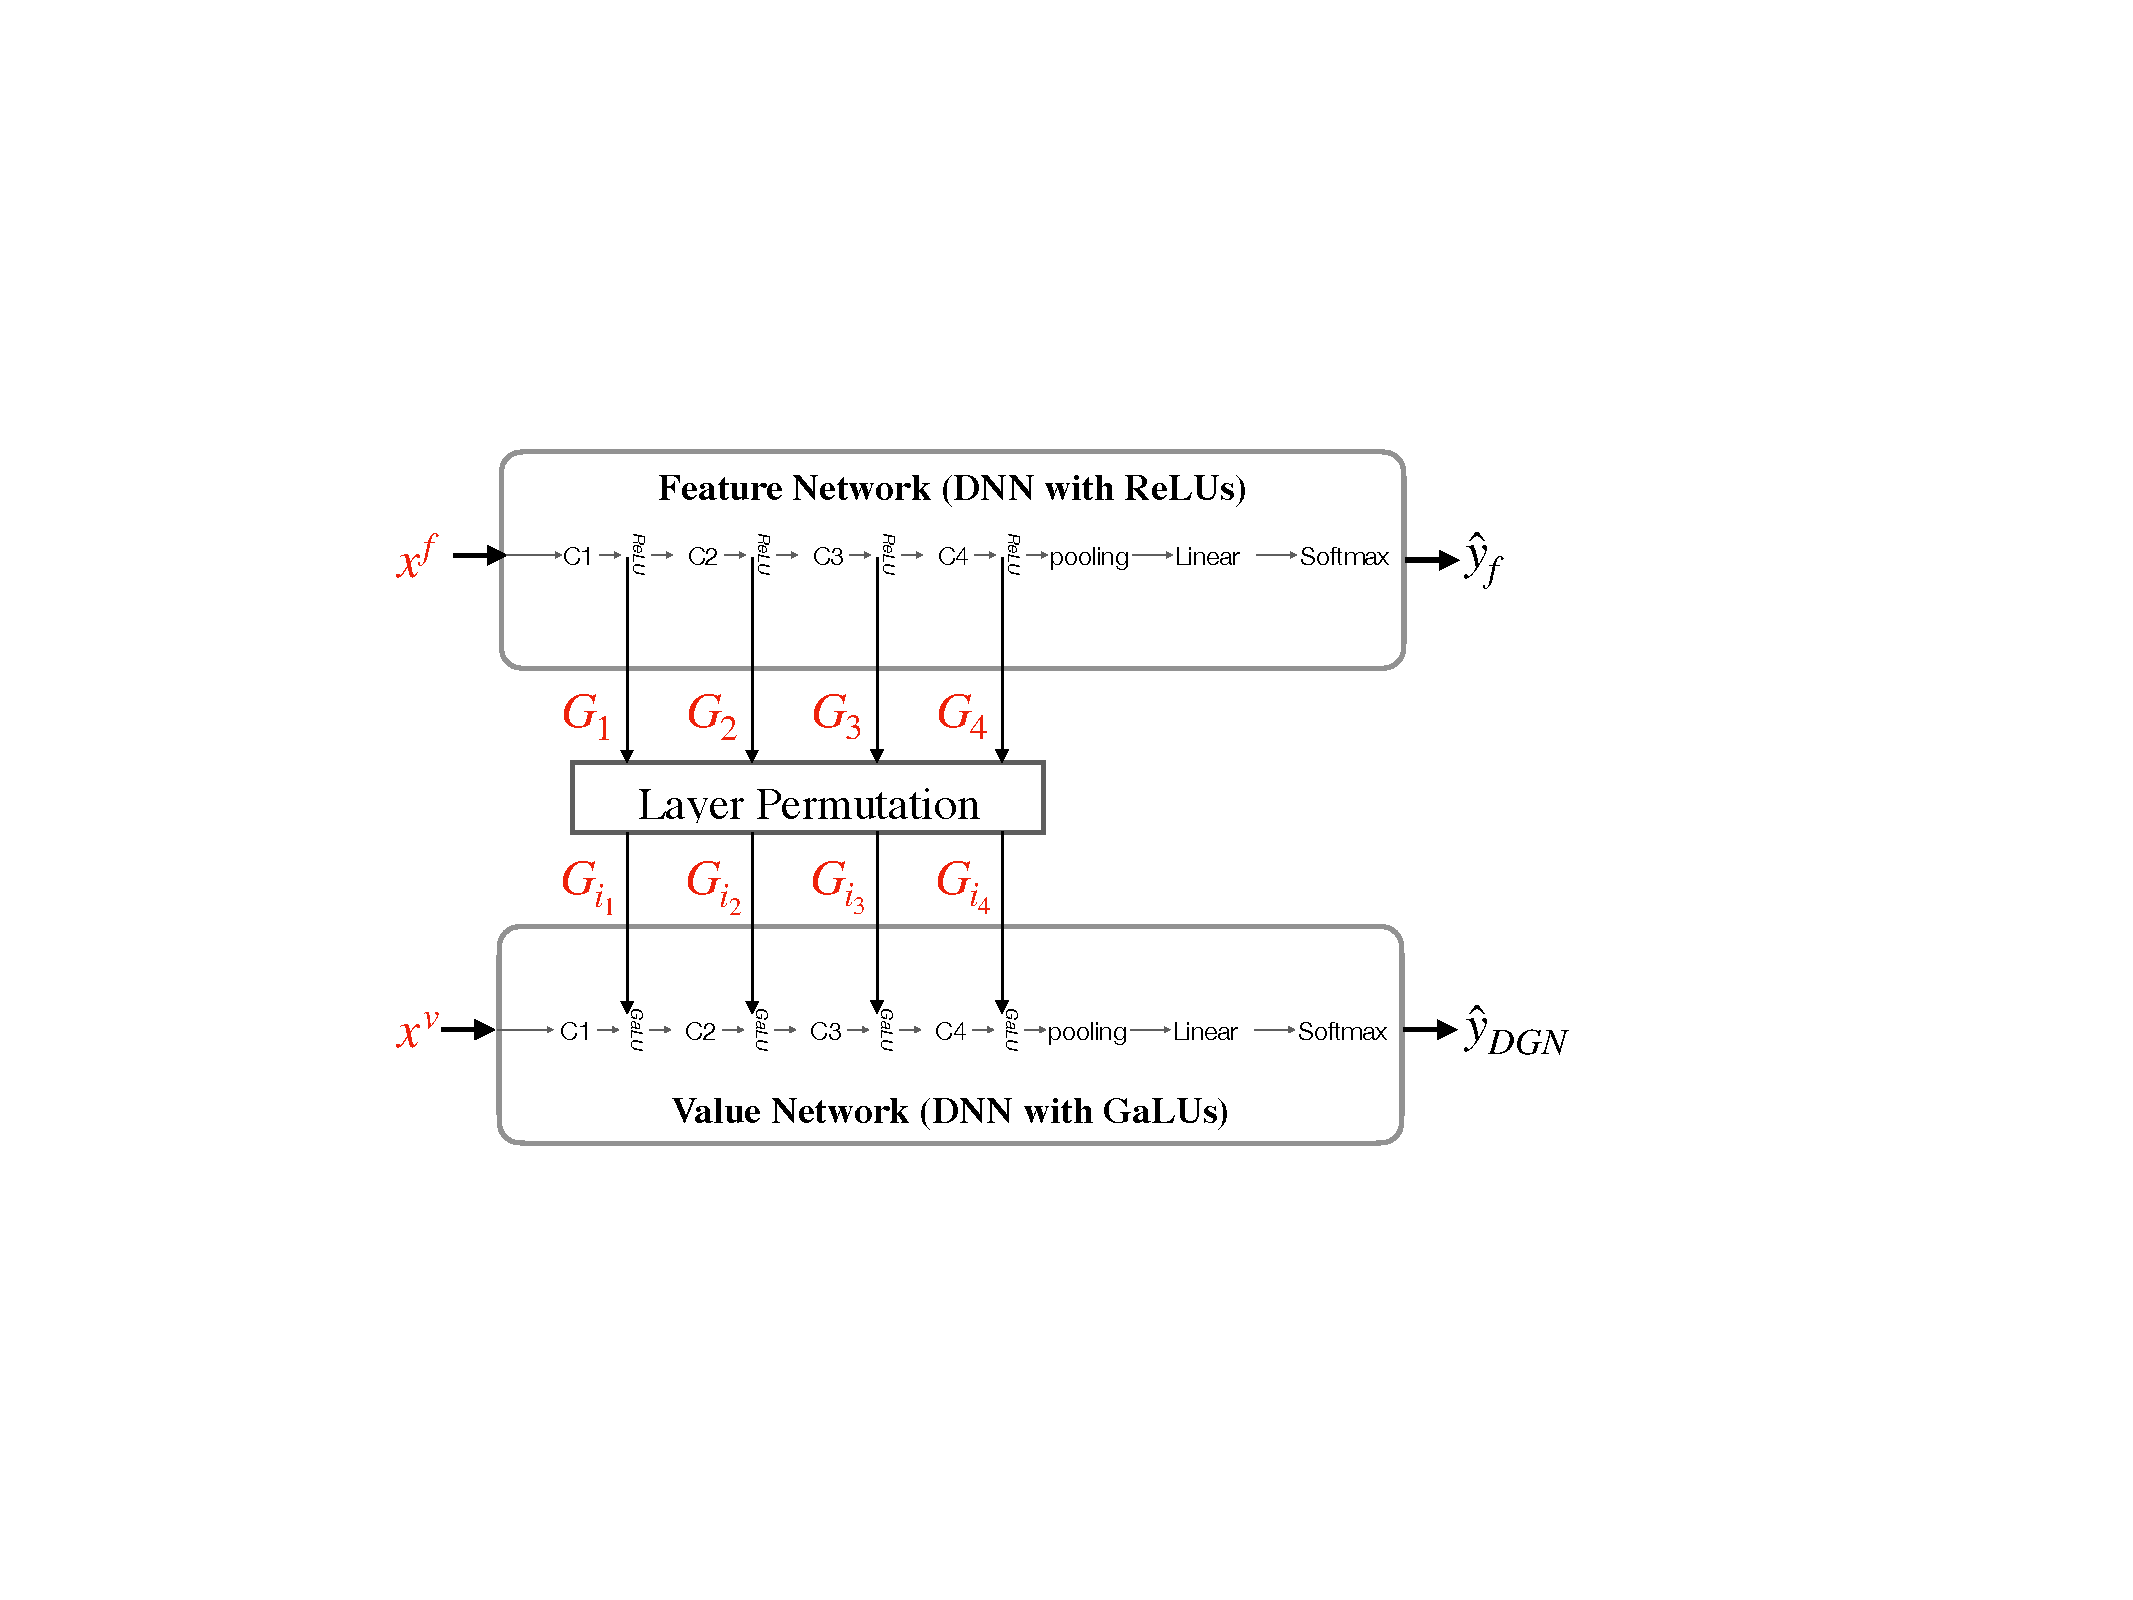
\includegraphics[scale=0.3]{figs/exp-new.pdf}
}
\end{minipage}
\caption{\small The prior setup in [\citenum{npk}] is shown in the left and the setup in this paper is shown in the right. Here $C1,\ldots,C4$ are convolutional layers with $128$ output filters, kernel size $3\times 3$ and stride $1\times 1$.}
\label{fig:dgn-prior-new}
\end{figure}
\begin{table}[t]
\centering
\begin{minipage}{0.95\columnwidth}
\begin{tabularx}{\columnwidth}{c *{5}{Y}}
\toprule
 Dataset& \multicolumn{2}{c}{Fixed Random}   &  \multicolumn{1}{c}{Decoupled} & \multicolumn{1}{c}{ Fixed } & \multicolumn{1}{c}{ReLU \tiny{(Feature Network)}}\\
& II & DI &Learning &Learnt &\\\hline\arrayrulecolor{white}\midrule
MNIST[\citenum{mnist}]& 94.1{\tiny{$\pm$0.3}}  &94.1\tiny{$\pm$0.3}  &98.1\tiny{$\pm$0.1} &98.6\tiny{$\pm$0.1} &98.5{\tiny{$\pm$0.1}}\\\hline\\\hline 
CIFAR-10[\citenum{cifar}]& 67.5\tiny{$\pm$0.7} &67.6\tiny{$\pm$0.7}   &77.6\tiny{$\pm$0.6} &79.4\tiny{$\pm$0.3} &80.4\tiny{$\pm$0.3}\\\hline
\arrayrulecolor{black}\bottomrule
\end{tabularx}
\end{minipage}
\caption{\small Shows the $\%$ test accuracy of various gates. The main result here is that the numbers in columns $1$ to $4$ are averaged over $48$ models (1 run per model, best performance in each run) and performance is robust to layer permutations and $x^{\text{v}}=\mathbf{1}$ input. For ReLU the average is over $5$ independent runs. Optimiser: Adam (3e-4). }
\label{tb:regimes}
\end{table}

\textbf{Note on prior results.} The following two observations were made in prior work [\citenum{npk}]: (i) by using the gates and training the NPV from scratch we can recover the performance (see ReLU vs Fixed Learnt in \Cref{tb:regimes}), and (ii) the performance of  Convolutional NTK ($77.43\%$)[\citenum{arora2019exact}] is between that of finite width network with random gates  ($67.5\%$) and learnt gates give ($79.4\%$), i.e., learning in the gates explains the difference between finite width DNNs and infinite width NTK.

\textbf{For `all-ones'} input to value network, in \Cref{th:main}, only $\ip{x,x'}=\din$, and $\Pi_{l=1}^{d-1}\frac{\ip{G_l(x),G_l(x')}}w$ is still unchanged. Similar explanations holds for \Cref{th:mainconv,th:mainres}.

\textbf{Robustness of Gates.} Entries in columns $1$ to $4$ in \Cref{tb:regimes} are  averaged over $48$ different models which included  permuting the layers and providing $\mathbf{1}$ as input. Our main result is that the information in the gates is robust over these $48$ models -- these justify the insights from \Cref{th:main} that as long as correlation in the gates is not destroyed the performance does not degrade. We also went one step further with respect to destroying the structure by considering arbitrary rotations. Here, we first tile the gates of the various filters (as a tensor) in the reverse order starting from layer $4$ to layer $1$ and then rotate arbitrarily in each of the three dimension for five times as shown in left of \Cref{fig:visual-permute} (i.e, two image dimensions and one filter dimension). For each rotation in the filter dimension we choose a random integer belonging to  $[0,512)$ and for each of the rotation in the image dimensions we choose a uniform random integer belonging to $[0,32)$. We did $10$ independent runs of the `fixed learnt' gates and `decoupled learning' of gates and observed the test performance to be $79.4${\tiny$\pm$0.2} and $79.0${\tiny$\pm$0.5} respectively (which are similar to the numbers shown in \Cref{tb:regimes}).

\begin{figure}[t]
\begin{minipage}{0.25\columnwidth}
\resizebox{\columnwidth}{!}{
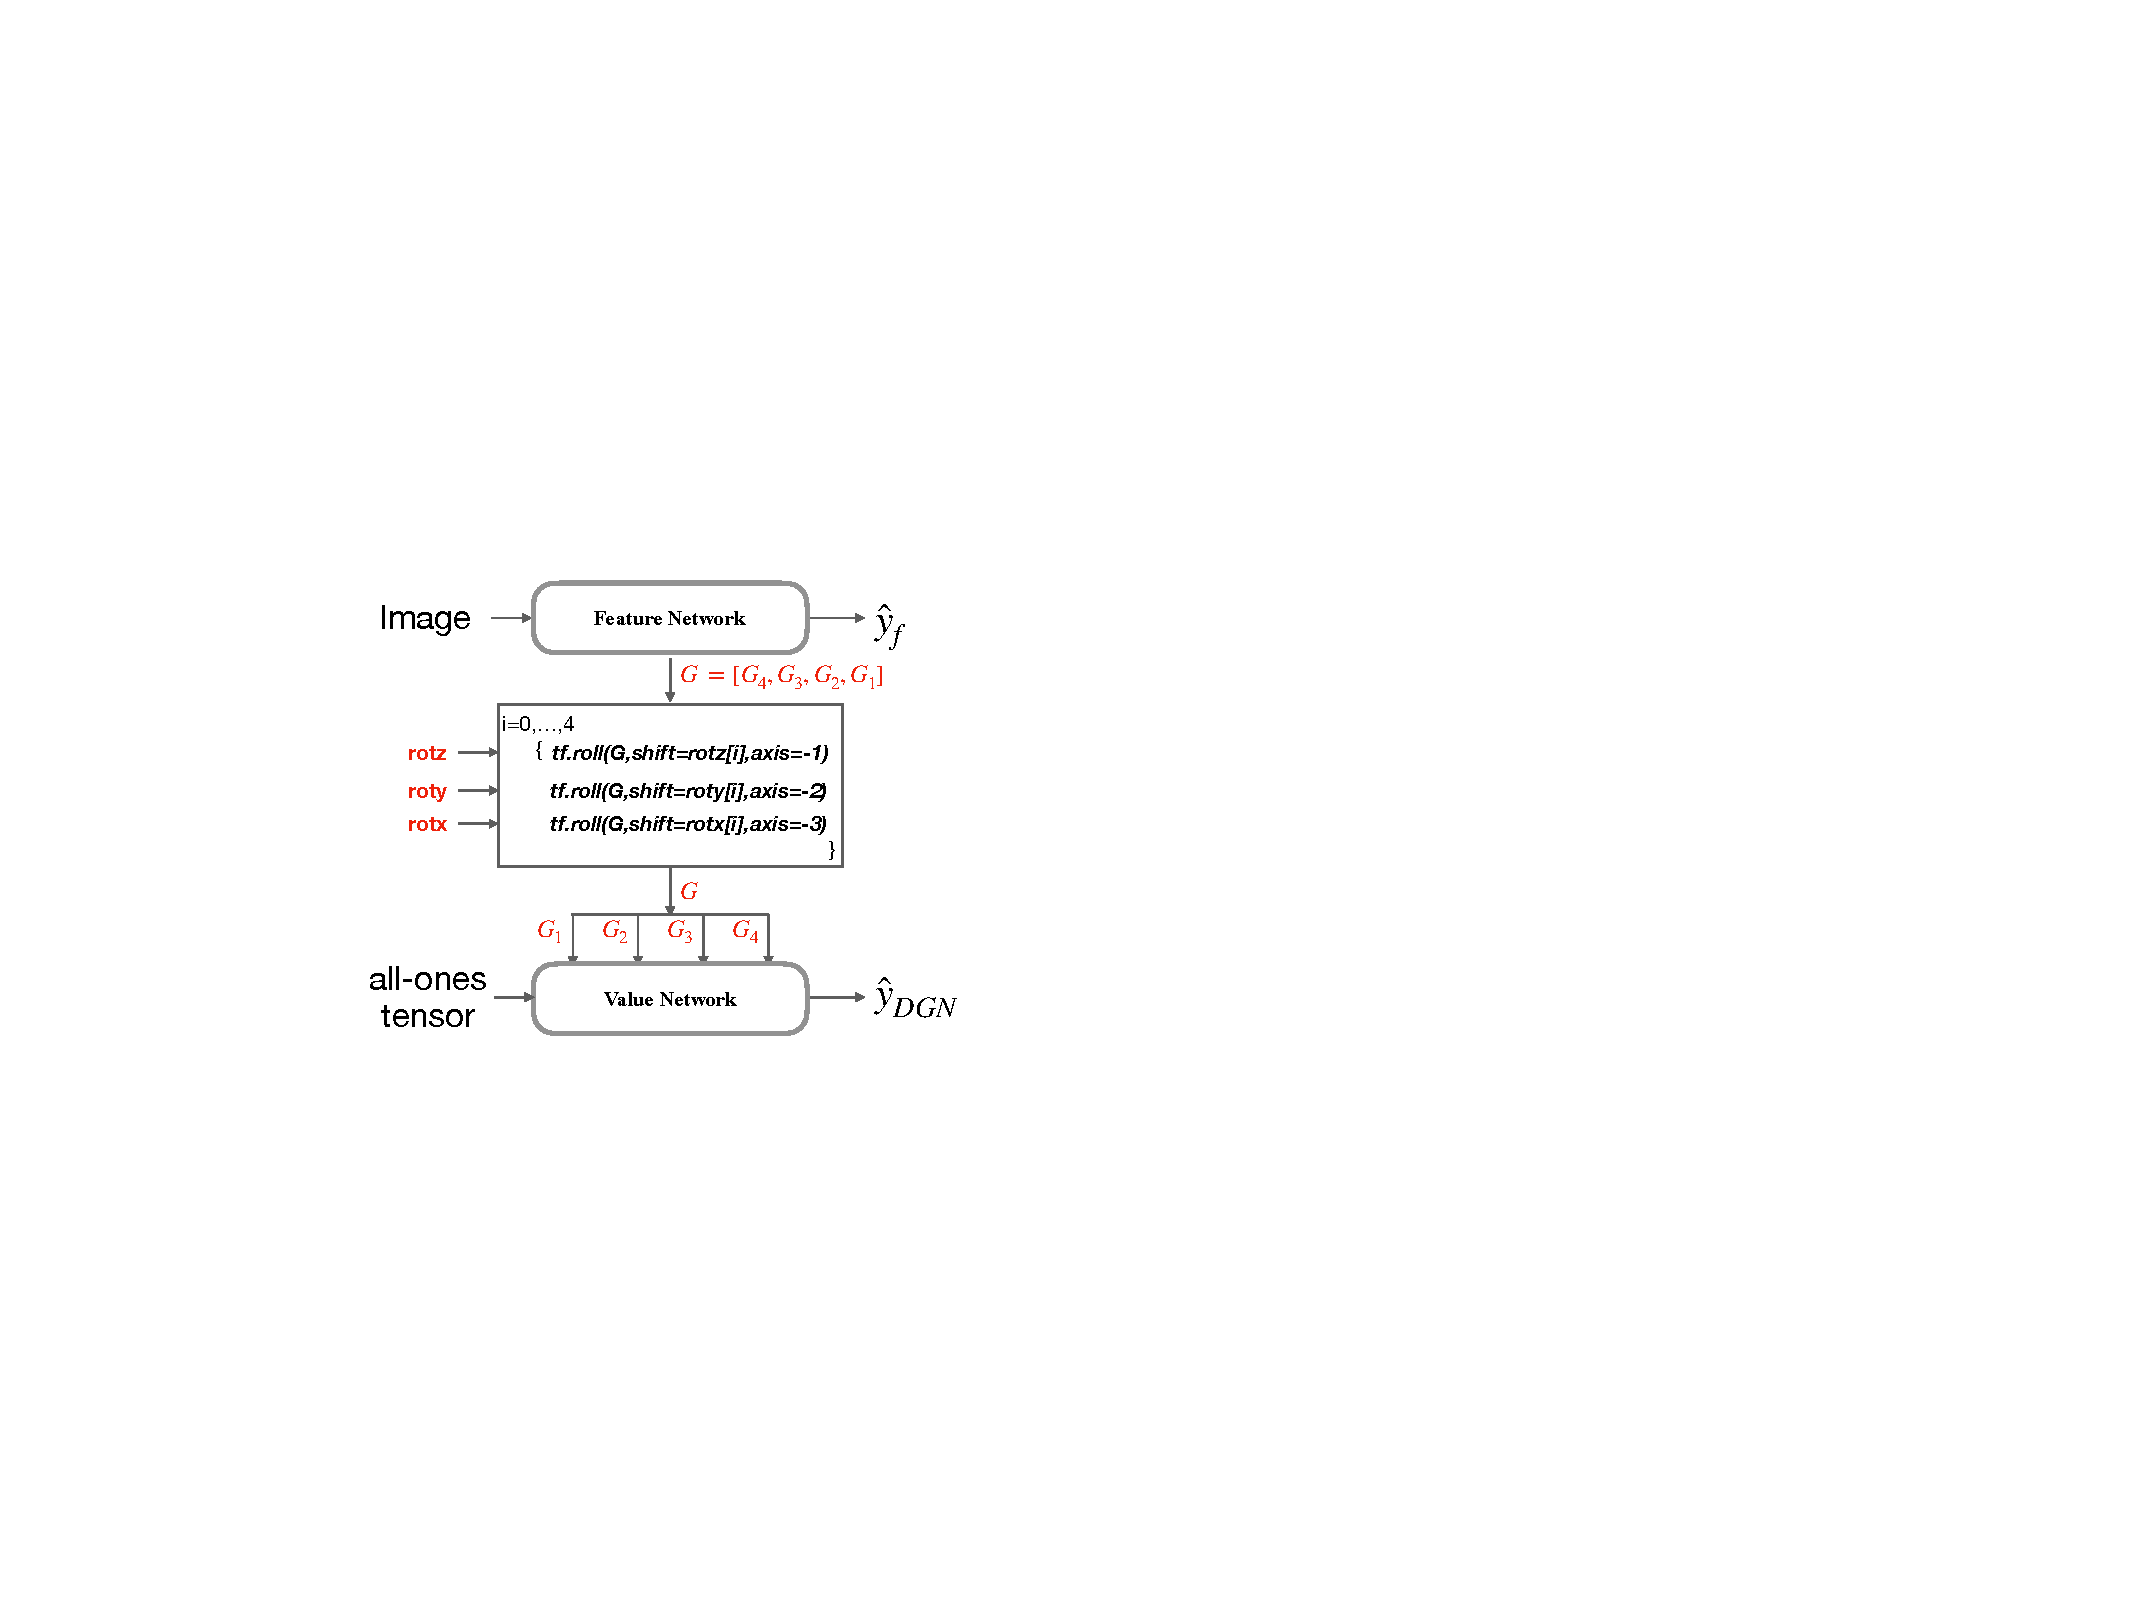
\includegraphics[scale=0.25]{figs/arbitrary_shift.pdf}
}
\end{minipage}
\begin{minipage}{0.68\columnwidth}
\resizebox{\columnwidth}{!}{
\begin{tabular}{c|c|cccccccc|c@{}}
&\resizebox{100pt}{!} {\Huge{Input}}& \resizebox{200pt}{!}{\Huge{Layer 1, Filter 1}}& \resizebox{200pt}{!}{\Huge{Layer 1, Filter 2}}&\resizebox{200pt}{!}{ \Huge{Layer 2, Filter 1}}& \resizebox{200pt}{!}{\Huge{Layer 2, Filter 2}}& \resizebox{200pt}{!}{\Huge{Layer 3, Filter 1}}& \resizebox{200pt}{!}{\Huge{Layer 3, Filter 2}}&\resizebox{200pt}{!}{\Huge{Layer 4, Filter 1}}& \resizebox{200pt}{!}{\Huge{Layer 4, Filter 2}}&\resizebox{180pt}{!}{\Huge{Test Acc.}}\\
\toprule
\resizebox{200pt}{!} {\shortstack{\Huge{Feature}\\\Huge Network\\\mbox{}\\\mbox{}\\\mbox{}\\\mbox{}\\\mbox{}\\\mbox{}\\\mbox{}}}&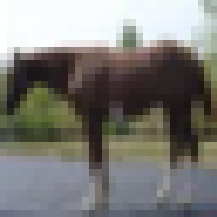
\includegraphics{visual-iclr/images/horse.png}&
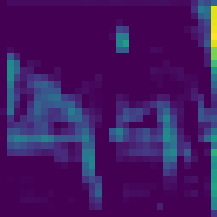
\includegraphics{images_neurips_2021/feature_network/layer_1_0.png}&
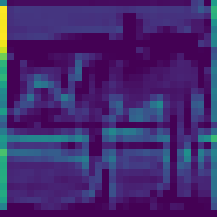
\includegraphics{images_neurips_2021/feature_network/layer_1_1.png}&
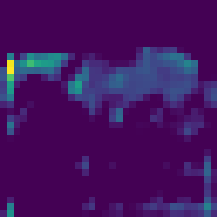
\includegraphics{images_neurips_2021/feature_network/layer_2_0.png}&
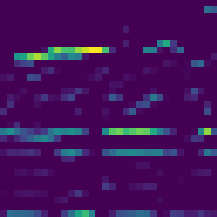
\includegraphics{images_neurips_2021/feature_network/layer_2_1.png}&
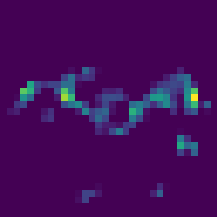
\includegraphics{images_neurips_2021/feature_network/layer_3_0.png}&
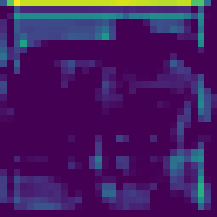
\includegraphics{images_neurips_2021/feature_network/layer_3_1.png}&
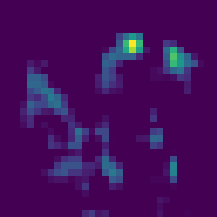
\includegraphics{images_neurips_2021/feature_network/layer_4_0.png}&
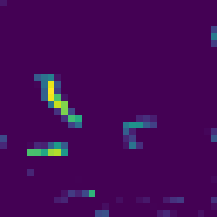
\includegraphics{images_neurips_2021/feature_network/layer_4_1.png}&
{\resizebox{200pt}{!}{\shortstack{80.4\tiny$\pm$0.3\\\mbox{}\\\mbox{}\\\mbox{}\\\mbox{}}} }\\\hline
\resizebox{200pt}{!} {\shortstack{\Huge{Value}\\\Huge Network\\\mbox{}\\\mbox{}\\\mbox{}\\\mbox{}\\\mbox{}\\\mbox{}\\\mbox{}}}&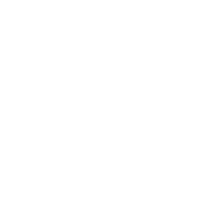
\includegraphics{images_neurips_2021/allones.png}&
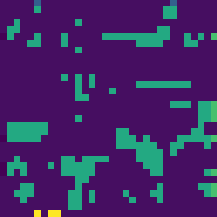
\includegraphics{images_neurips_2021/value_network//layer_1_0.png}&
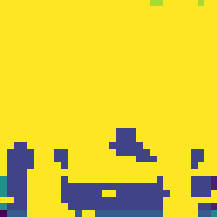
\includegraphics{images_neurips_2021/value_network//layer_1_1.png}&
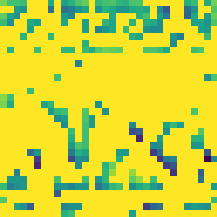
\includegraphics{images_neurips_2021/value_network//layer_2_0.png}&
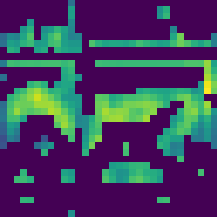
\includegraphics{images_neurips_2021/value_network//layer_2_1.png}&
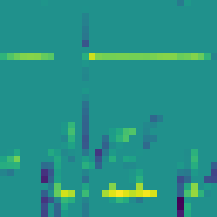
\includegraphics{images_neurips_2021/value_network//layer_3_0.png}&
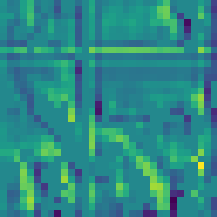
\includegraphics{images_neurips_2021/value_network//layer_3_1.png}&
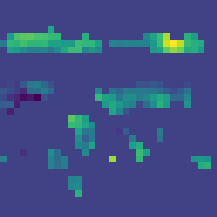
\includegraphics{images_neurips_2021/value_network//layer_4_0.png}&
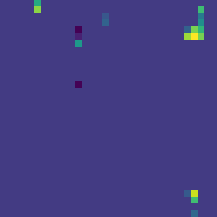
\includegraphics{images_neurips_2021/value_network//layer_4_1.png}&
{\resizebox{200pt}{!}{\shortstack{79.4 \tiny$\pm$0.2\\\mbox{}\\\mbox{}\\\mbox{}\\\mbox{}}} }\\
\end{tabular}
}

\end{minipage}
\caption{\small On the left is the setup for arbitrary rotation of gates. On the right, we have the images related to feature and value networks on top and bottom rows respectively. Each row has the input image followed by the output of first $2$ filters in each of the $4$ layers.  In the bottom row, the input column `appears' blank because it is the image of the $\mathbf{1}$ input to the value network.  Despite the arbitrary rotation and $\mathbf{1}$ input,  the value network is within $1\%$ of  feature network's test accuracy (on CIFAR-10).}
\label{fig:visual-permute}
\end{figure}

\textbf{Primal vs Dual View of features.} The standard (primal) view is that the input is processed layer-by-layer and the hidden features are in the layer outputs. 
%The dual view is that the features are encoded in the gates (analytically speaking the NPF/NPK). While both are mathematically equivalent, we believe that the dual view paints more accurate picture. 
Our experiments challenge the primal view, because, 
we do not provide the image as input but only $\mathbf{1}$ (`all-ones') as input to the value network, and we have destroyed the layer-by-layer structure of the gates before applying them as masks in the value network as well (also, the `fixed learnt' gates do not change during training). As a result, there is a huge `visual' difference between the hidden layer outputs of the feature network and that of the value network (see right of \Cref{fig:visual-permute}).  One could still insist that DNNs are so powerful that they are recovering the features layer-by-layer. Or alternatively, one can appeal to the dual view to conclude that since neither `all-ones' input nor the arbitrary rotation of the gates affect the correlation of gates (\Cref{th:main}), the performance does not degrade. While the gates are generated layer-by-layer in the feature network, when applied as masks, the function of the gates is to select and train the sub-networks corresponding to each example (viewpoint trivially following from \Cref{prop:npf-npv}) .
\begin{comment}
\textbf{Primal vs Dual View of features.} The standard (primal) view is that the input is processed layer-by-layer and the hidden features are in the layer outputs. To challenge this view, 
%The dual view is that the features are encoded in the gates (analytically speaking the NPF/NPK). While both are mathematically equivalent, we believe that the dual view paints more accurate picture. Our experiments challenge the primal view. 
we do not provide the image as input but only $\mathbf{1}$ (`all-ones') as input to the value network. Now, it could be argued that the value network gets the information about the via its gating masks. To counter this argument, we have destroyed the layer-by-layer structure of the gates before applying them as masks in the value network as well. As a result, there is a huge `visual' difference between the hidden layer outputs of the feature network and that of the value network (see right of \Cref{fig:visual-permute}).  One could still insist that DNNs are so powerful that they are recovering the features layer-by-layer. Or alternatively, one can appeal to the dual view to conclude that since neither `all-ones' input nor the arbitrary rotation of the gates affect the correlation of gates (\Cref{th:main}), the performance does not degrade. While the gates are generated layer-by-layer in the feature network, when applied as masks, the function of the gates is to learn and train the paths and sub-networks (viewpoint trivially following from \Cref{prop:npf-npv}) .
\end{comment}

\textbf{Gate learning need not be layer-by-layer.} In `decoupled learning' (\Cref{tb:regimes}), while the gates are generated layer-by-layer in the feature network, after arbitrary rotations they end in a different location in the value network during training, i.e., the gates can be arbitrarily placed while learning.




\begin{comment}
\begin{figure}
\centering
\begin{minipage}{1.0\columnwidth}
\begin{minipage}{1.0\columnwidth}
\resizebox{0.99\columnwidth}{!}{
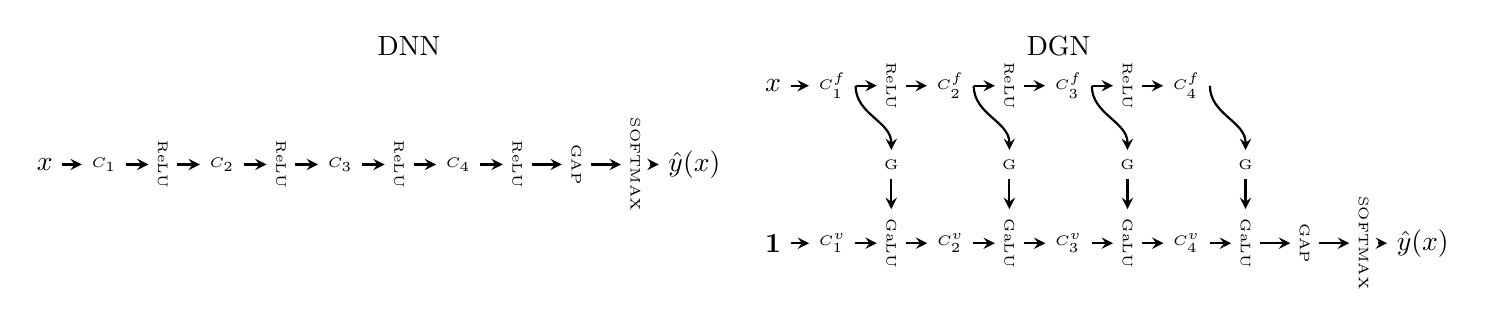
\begin{tikzpicture}
\node []  (dnn-text)at (-4.125,2) {DNN};

\node []  (dnn-output) at (-0.5,0.5) {$\hat{y}(x)$};
\node [rotate=-90]  (dnn-smax) at (-1.25,0.5) {\tiny{SOFTMAX}};
\draw [-stealth,thick]   (dnn-smax.north) -- (dnn-output.west);

\node [rotate=-90]  (dnn-gap) at (-2,0.5) {\tiny{GAP}};
\draw [-stealth,thick]   (dnn-gap.north) -- (dnn-smax.south);

\node [rotate=-90] (dnn-relu-4) at (-2.75,0.5){\tiny{ReLU}};
\node [] (dnn-c4) at (-3.5,0.5){\tiny{$C_4$}};
\draw [-stealth,thick]   (dnn-c4.east) -- (dnn-relu-4.south);
\draw [-stealth,thick]   (dnn-relu-4.north) -- (dnn-gap.south);



\node [rotate=-90] (dnn-relu-3) at (-4.25,0.5){\tiny{ReLU}};
\node [] (dnn-c3) at (-5,0.5){\tiny{$C_3$}};
\draw [-stealth,thick]   (dnn-c3.east) -- (dnn-relu-3.south);
\draw [-stealth,thick]   (dnn-relu-3.north) -- (dnn-c4.west);


\node [rotate=-90] (dnn-relu-2) at (-5.75,0.5){\tiny{ReLU}};
\node [] (dnn-c2) at (-6.5,0.5){\tiny{$C_2$}};
\draw [-stealth,thick]   (dnn-c2.east) -- (dnn-relu-2.south);
\draw [-stealth,thick]   (dnn-relu-2.north) -- (dnn-c3.west);

\node [rotate=-90] (dnn-relu-1) at (-7.25,0.5){\tiny{ReLU}};
\node [] (dnn-c1) at (-8,0.5){\tiny{$C_1$}};
\draw [-stealth,thick]   (dnn-c1.east) -- (dnn-relu-1.south);
\draw [-stealth,thick]   (dnn-relu-1.north) -- (dnn-c2.west);



\node [] (dnn-input) at (-8.75,0.5){$x$};
\draw [-stealth,thick]   (dnn-input.east) -- (dnn-c1.west);


%%%%%%%%%%%%%%%%%%%%%%%%%%%%%%%%%%%%%%%%%%%%%%%%%%%%%%%%%%%%%%%%%
\node []  (fntext)at (4.125,2) {DGN};

%\node []  (output) at (7.5,1.5) {$\hat{y}(x)$};


\node [] (dgn-f-c4) at (5.75,1.5){\tiny{$C^{\text{f}}_4$}};


\node [rotate=-90] (dgn-relu-3) at (5,1.5){\tiny{ReLU}};
\node [] (dgn-f-c3) at (4.25,1.5){\tiny{$C^{\text{f}}_3$}};
\draw [-stealth,thick]   (dgn-f-c3.east) -- (dgn-relu-3.south);
\draw [-stealth,thick]   (dgn-relu-3.north) -- (dgn-f-c4.west);


\node [rotate=-90] (dgn-relu-2) at (3.5,1.5){\tiny{ReLU}};
\node [] (dgn-f-c2) at (2.75,1.5){\tiny{$C^{\text{f}}_2$}};
\draw [-stealth,thick]   (dgn-f-c2.east) -- (dgn-relu-2.south);
\draw [-stealth,thick]   (dgn-relu-2.north) -- (dgn-f-c3.west);


\node [rotate=-90] (dgn-relu-1) at (2,1.5){\tiny{ReLU}};
\node [] (dgn-f-c1) at (1.25,1.5){\tiny{$C^{\text{f}}_1$}};
\draw [-stealth,thick]   (dgn-f-c1.east) -- (dgn-relu-1.south);
\draw [-stealth,thick]   (dgn-relu-1.north) -- (dgn-f-c2.west);



\node [] (dgn-f-input) at (0.5,1.5){$x$};
\draw [-stealth,thick]   (dgn-f-input.east) -- (dgn-f-c1.west);

\node []  (dgn-output) at (8.75,-0.5) {$\hat{y}(x)$};
\node [rotate=-90] (dgn-smax) at (8,-0.5){\tiny{SOFTMAX}};
\draw [-stealth,thick]   (dgn-smax.north)--(dgn-output.west);

\node [rotate=-90] (dgn-gap) at (7.25,-0.5){\tiny{GAP}};
\draw [-stealth,thick]   (dgn-gap.north)--(dgn-smax.south);



\node [rotate=-90] (dgn-galu-4) at (6.5,-0.5){\tiny{GaLU}};
\draw [-stealth,thick]   (dgn-galu-4.north) -- (dgn-gap.south);

\node [] (dgn-v-c4) at (5.75,-0.5){\tiny{$C^{\text{v}}_4$}};
\draw [-stealth,thick]   (dgn-v-c4.east) -- (dgn-galu-4.south);

\node [rotate=-90] (dgn-galu-3) at (5,-0.5){\tiny{GaLU}};
\node [] (dgn-v-c3) at (4.25,-0.5){\tiny{$C^{\text{v}}_3$}};
\draw [-stealth,thick]   (dgn-v-c3.east) -- (dgn-galu-3.south);
\draw [-stealth,thick]   (dgn-galu-3.north) -- (dgn-v-c4.west);



\node [rotate=-90] (dgn-galu-2) at (3.5,-0.5){\tiny{GaLU}};
\node [] (dgn-v-c2) at (2.75,-0.5){\tiny{$C^{\text{v}}_2$}};
\draw [-stealth,thick]   (dgn-v-c2.east) -- (dgn-galu-2.south);
\draw [-stealth,thick]   (dgn-galu-2.north) -- (dgn-v-c3.west);


\node [rotate=-90] (dgn-galu-1) at (2,-0.5){\tiny{GaLU}};
\node [] (dgn-v-c1) at (1.25,-0.5){\tiny{$C^{\text{v}}_1$}};

\draw [-stealth,thick]   (dgn-v-c1.east) -- (dgn-galu-1.south);
\draw [-stealth,thick]   (dgn-galu-1.north) -- (dgn-v-c2.west);




\node [] (dgn-input) at (0.5,-0.5){$\mathbf{1}$};
\draw [-stealth,thick]   (dgn-input.east) -- (dgn-v-c1.west);




\node[] (dgn-gating-1) at (2,0.5){\tiny{G}};
\draw [-stealth,thick]   (dgn-f-c1.east) to[out=-90,in=90] (dgn-gating-1.north);
\draw [-stealth,thick]   (dgn-gating-1.south) -- (dgn-galu-1.west);


\node[] (dgn-gating-2) at (3.5,0.5){\tiny{G}};
\draw [-stealth,thick]   (dgn-f-c2.east) to[out=-90,in=90] (dgn-gating-2.north);
\draw [-stealth,thick]   (dgn-gating-2.south) -- (dgn-galu-2.west);



\node[] (dgn-gating-3) at (5,0.5){\tiny{G}};
\draw [-stealth,thick]   (dgn-f-c3.east) to[out=-90,in=90] (dgn-gating-3.north);
\draw [-stealth,thick]   (dgn-gating-3.south) -- (dgn-galu-3.west);


\node[] (dgn-gating-4) at (6.5,0.5){\tiny{G}};
\draw [-stealth,thick]   (dgn-f-c4.east) to[out=-90,in=90] (dgn-gating-4.north);
\draw [-stealth,thick]   (dgn-gating-4.south) -- (dgn-galu-4.west);

	
\end{tikzpicture}


}
\end{minipage}
\begin{minipage}{1.0\columnwidth}
\resizebox{0.99\columnwidth}{!}{
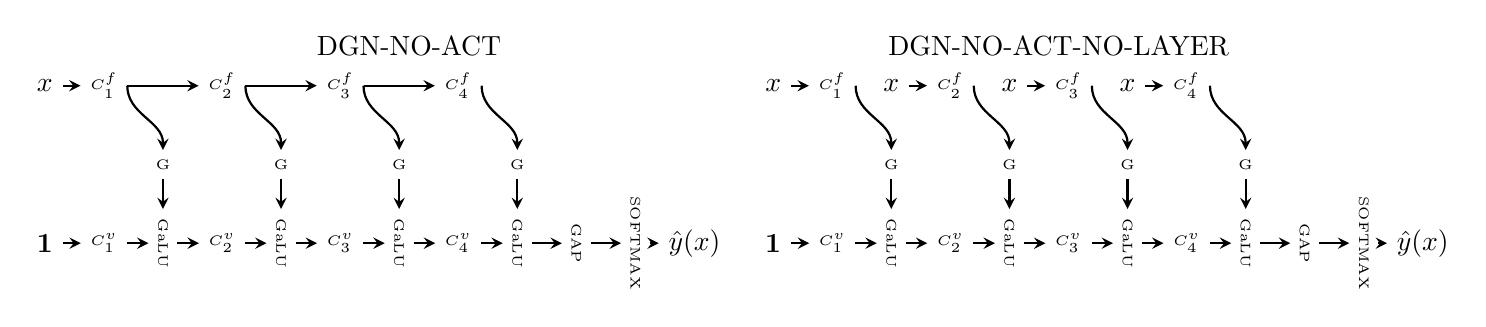
\begin{tikzpicture}
\node []  (fntext)at (-4.125,2) {DGN-NO-ACT};

%\node []  (output) at (7.5,1.5) {$\hat{y}(x)$};


\node [] (dgn1-f-c4) at (-3.5,1.5){\tiny{$C^{\text{f}}_4$}};
\node [] (dgn1-f-c3) at (-5,1.5){\tiny{$C^{\text{f}}_3$}};
\node [] (dgn1-f-c2) at (-6.5,1.5){\tiny{$C^{\text{f}}_2$}};
\node [] (dgn1-f-c1) at (-8,1.5){\tiny{$C^{\text{f}}_1$}};
\node [] (dgn1-input-f) at (-8.75,1.5){$x$};
\draw [-stealth,thick]   (dgn1-f-c3.east) -- (dgn1-f-c4.west);
\draw [-stealth,thick]   (dgn1-f-c2.east) -- (dgn1-f-c3.west);
\draw [-stealth,thick]   (dgn1-f-c1.east) -- (dgn1-f-c2.west);
\draw [-stealth,thick]   (dgn1-input-f.east) -- (dgn1-f-c1.west);



\node []  (dgn1-output) at (-0.5,-0.5) {$\hat{y}(x)$};

\node [rotate=-90] (dgn1-smax) at (-1.25,-0.5){\tiny{SOFTMAX}};
\draw [-stealth,thick]   (dgn1-smax.north)--(dgn1-output.west);

\node [rotate=-90] (dgn1-gap) at (-2,-0.5){\tiny{GAP}};
\draw [-stealth,thick]   (dgn1-gap.north)--(dgn1-smax.south);


\node [rotate=-90] (dgn1-galu-4) at (-2.75,-0.5){\tiny{GaLU}};
\draw [-stealth,thick]   (dgn1-galu-4.north)--(dgn1-gap.south);

\node [] (dgn1-v-c4) at (-3.5,-0.5){\tiny{$C^{\text{v}}_4$}};
\draw [-stealth,thick]   (dgn1-v-c4.east) -- (dgn1-galu-4.south);


\node [rotate=-90] (dgn1-galu-3) at (-4.25,-0.5){\tiny{GaLU}};
\draw [-stealth,thick]   (dgn1-galu-3.north) -- (dgn1-v-c4.west);

\node [] (dgn1-v-c3) at (-5,-0.5){\tiny{$C^{\text{v}}_3$}};
\draw [-stealth,thick]   (dgn1-v-c3.east) -- (dgn1-galu-3.south);


\node [rotate=-90] (dgn1-galu-2) at (-5.75,-0.5){\tiny{GaLU}};
\draw [-stealth,thick]   (dgn1-galu-2.north) -- (dgn1-v-c3.west);

\node [] (dgn1-v-c2) at (-6.5,-0.5){\tiny{$C^{\text{v}}_2$}};
\draw [-stealth,thick]   (dgn1-v-c2.east) -- (dgn1-galu-2.south);


\node [rotate=-90] (dgn1-galu-1) at (-7.25,-0.5){\tiny{GaLU}};
\draw [-stealth,thick]   (dgn1-galu-1.north) -- (dgn1-v-c2.west);


\node [] (dgn1-v-c1) at (-8,-0.5){\tiny{$C^{\text{v}}_1$}};
\draw [-stealth,thick]   (dgn1-v-c1.east) -- (dgn1-galu-1.south);


\node [] (dgn1-v-input) at (-8.75,-0.5){$\mathbf{1}$};




\node[] (dgn1-gating-4) at (-2.75,0.5){\tiny{G}};
\node[] (dgn1-gating-3) at (-4.25,0.5){\tiny{G}};
\node[] (dgn1-gating-2) at (-5.75,0.5){\tiny{G}};
\node[] (dgn1-gating-1) at (-7.25,0.5){\tiny{G}};

\draw [-stealth,thick]   (dgn1-f-c1.east) to[out=-90,in=90] (dgn1-gating-1.north);
\draw [-stealth,thick]   (dgn1-gating-1.south) -- (dgn1-galu-1.west);



\draw [-stealth,thick]   (dgn1-f-c2.east) to[out=-90,in=90] (dgn1-gating-2.north);
\draw [-stealth,thick]   (dgn1-gating-2.south) -- (dgn1-galu-2.west);




\draw [-stealth,thick]   (dgn1-f-c3.east) to[out=-90,in=90] (dgn1-gating-3.north);
\draw [-stealth,thick]   (dgn1-gating-3.south) -- (dgn1-galu-3.west);



\draw [-stealth,thick]   (dgn1-f-c4.east) to[out=-90,in=90] (dgn1-gating-4.north);
\draw [-stealth,thick]   (dgn1-gating-4.south) -- (dgn1-galu-4.west);

\draw [-stealth,thick]   (dgn1-v-input.east) -- (dgn1-v-c1.west);

%%%%%%%%%%%%%%%%%%%%%%%%%%%%%%%%%%%%%%%%%%%%%%%%%%%%%%%%%%%%%%%%%
\node []  (fntext)at (4.125,2) {DGN-NO-ACT-NO-LAYER};

%\node []  (output) at (7.5,1.5) {$\hat{y}(x)$};

\node [] (dgn-f-input) at (0.5,1.5){$x$};
\node [] (dgn-f-c4) at (5.75,1.5){\tiny{$C^{\text{f}}_4$}};

\node [] (dgn-f-x-4) at (5,1.5){$x$};


\node [] (dgn-f-c3) at (4.25,1.5){\tiny{$C^{\text{f}}_3$}};
\node [] (dgn-f-x-3) at (3.5,1.5){$x$};

\node [] (dgn-f-c2) at (2.75,1.5){\tiny{$C^{\text{f}}_2$}};
\node [] (dgn-f-x-2) at (2,1.5){$x$};

\node [] (dgn-f-c1) at (1.25,1.5){\tiny{$C^{\text{f}}_1$}};

\draw [-stealth,thick]   (dgn-f-input.east) -- (dgn-f-c1.west);
\draw [-stealth,thick]   (dgn-f-x-2.east) -- (dgn-f-c2.west);
\draw [-stealth,thick]   (dgn-f-x-3.east) -- (dgn-f-c3.west);
\draw [-stealth,thick]   (dgn-f-x-4.east) -- (dgn-f-c4.west);


\node []  (dgn-output) at (8.75,-0.5) {$\hat{y}(x)$};



\node [rotate=-90] (dgn-smax) at (8,-0.5){\tiny{SOFTMAX}};
\draw [-stealth,thick]   (dgn-smax.north) -- (dgn-output.west);
;
\node [rotate=-90] (dgn-gap) at (7.25,-0.5){\tiny{GAP}};
\draw [-stealth,thick]   (dgn-gap.north) -- (dgn-smax.south);



\node [rotate=-90] (dgn-galu-4) at (6.5,-0.5){\tiny{GaLU}};

\draw [-stealth,thick]   (dgn-galu-4.north) -- (dgn-gap.south);
\node [] (dgn-v-c4) at (5.75,-0.5){\tiny{$C^{\text{v}}_4$}};
\draw [-stealth,thick]   (dgn-v-c4.east) -- (dgn-galu-4.south);


\node [rotate=-90] (dgn-galu-3) at (5,-0.5){\tiny{GaLU}};
\draw [-stealth,thick]   (dgn-galu-3.north) -- (dgn-v-c4.west);


\node [] (dgn-v-c3) at (4.25,-0.5){\tiny{$C^{\text{v}}_3$}};
\draw [-stealth,thick]   (dgn-v-c3.east) -- (dgn-galu-3.south);


\node [rotate=-90] (dgn-galu-2) at (3.5,-0.5){\tiny{GaLU}};
\draw [-stealth,thick]   (dgn-galu-2.north) -- (dgn-v-c3.west);

\node [] (dgn-v-c2) at (2.75,-0.5){\tiny{$C^{\text{v}}_2$}};
\draw [-stealth,thick]   (dgn-v-c2.east) -- (dgn-galu-2.south);


\node [rotate=-90] (dgn-galu-1) at (2.0,-0.5){\tiny{GaLU}};
\draw [-stealth,thick]   (dgn-galu-1.north) -- (dgn-v-c2.west);

\node [] (dgn-v-c1) at (1.25,-0.5){\tiny{$C^{\text{v}}_1$}};
\draw [-stealth,thick]   (dgn-v-c1.east) -- (dgn-galu-1.south);


\node [] (dgn-v-input) at (0.5,-0.5){$\mathbf{1}$};


\node[] (dgn-gating-1) at (2.0,0.5){\tiny{G}};
\draw [-stealth,thick]   (dgn-f-c1.east) to[out=-90,in=90] (dgn-gating-1.north);
\draw [-stealth,thick]   (dgn-gating-1.south) -- (dgn-galu-1.west);


\node[] (dgn-gating-2) at (3.5,0.5){\tiny{G}};
\draw [-stealth,thick]   (dgn-f-c2.east) to[out=-90,in=90] (dgn-gating-2.north);
\draw [-stealth,thick]   (dgn-gating-2.south) -- (dgn-galu-2.west);



\node[] (dgn-gating-3) at (5,0.5){\tiny{G}};
\draw [-stealth,thick]   (dgn-f-c3.east) to[out=-90,in=90] (dgn-gating-3.north);
\draw [-stealth,thick]   (dgn-gating-3.south) -- (dgn-galu-3.west);


\node[] (dgn-gating-4) at (6.5,0.5){\tiny{G}};
\draw [-stealth,thick]   (dgn-f-c4.east) to[out=-90,in=90] (dgn-gating-4.north);
\draw [-stealth,thick]   (dgn-gating-4.south) -- (dgn-galu-4.west);

\draw [-stealth,thick]   (dgn-v-input.east) -- (dgn-v-c1.west);
	
\end{tikzpicture}


}
\end{minipage}
\end{minipage}
\caption{$4$ convolutional layers with GAP}
\label{fig:c4gap}
\end{figure}
\end{comment}
